%\subsection{3D Visualization}

%\frame
%{
%   \frametitle{3D Visualization - Description}
%
%   \includegraphics[width=\textwidth]{img/simple-appgraph.pdf} 
%   \vfill
%   \includegraphics[width=\textwidth]{img/simple-resgraph.pdf}
%}


\frame
{
   \frametitle{3D Visualization - Communication Patterns}

   \begin{itemize}
   \item Differences from the space-time diagram
   \end{itemize}

   \vfill
   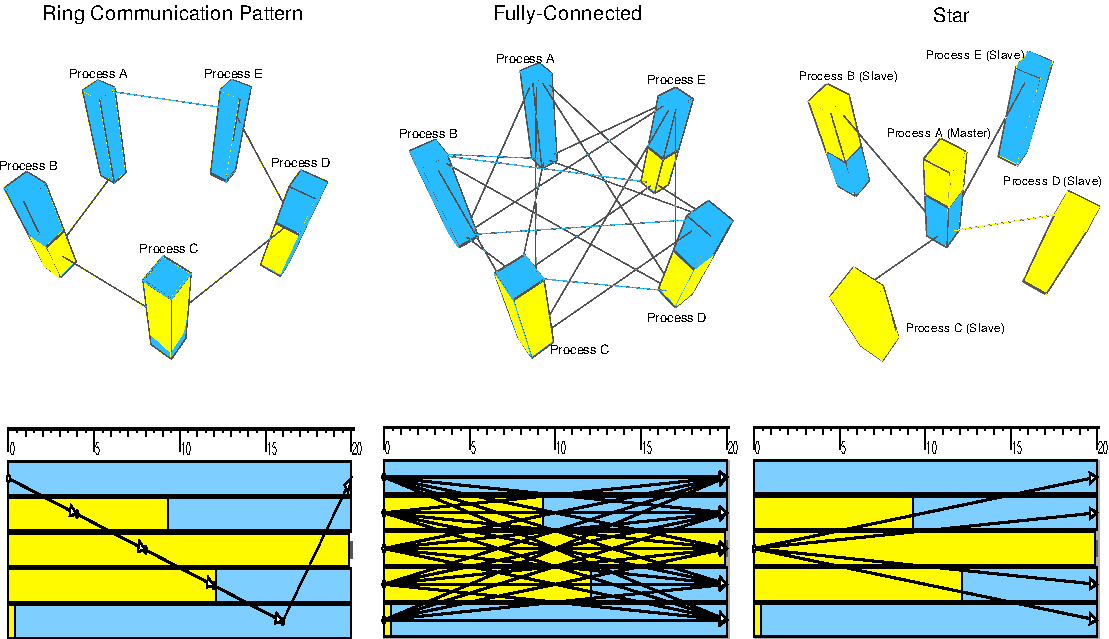
\includegraphics[width=\textwidth]{img/apppattern-ring-full-star.pdf}
   \vfill
}


\frame
{
   \frametitle{3D Visualization - KAAPI Trace}
   \begin{itemize}
   \item Fibonacci Application
   \item 26 processes, two sites, two clusters
   \item Lines represent steal requests
   \item Different number of communication between clusters
      \begin{itemize}
      \item beggining $\rightarrow$ big tasks, less communication
      \item end $\rightarrow$ smaller tasks, more communication
      \end{itemize}
   \end{itemize}

   \vfill
   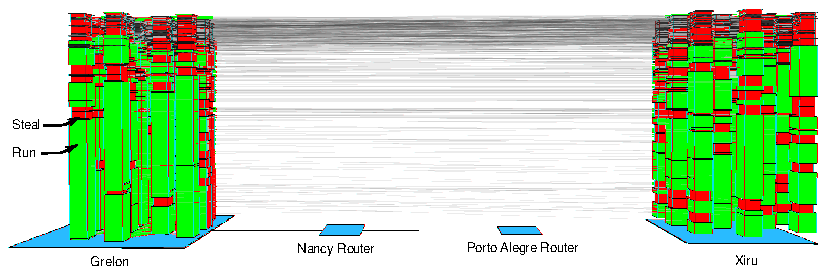
\includegraphics[width=\textwidth]{img/scenario-3d-A2.pdf}
}

\frame
{
   \frametitle{3D Visualization - KAAPI Trace}
   \begin{itemize}
   \item 60 processes, two sites, three clusters
%   \item Dashed line depicts the site separation
   \item Total execution time of a KAAPI fibonacci application
   \item Observe number of requests in time
%   \item Right image shows a larger time scale
%   \item All steal requests must go through two routers
%   \item Different stealing behavior in different intervals of time
%   \item Beggining $\rightarrow$ less requests, End $\rightarrow$ More requests
%   \item Expected behavior
   \end{itemize}

   \vfill
   \hspace{-1cm}
   \begin{minipage}{\textwidth}
   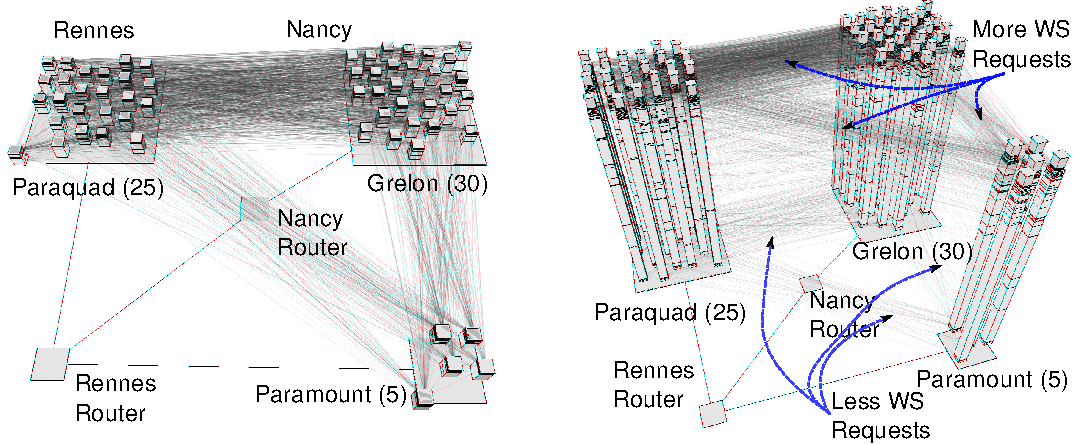
\includegraphics[width=1.15\textwidth]{img/scenario-3d-A.pdf}
   \end{minipage}
}


%\frame
%{
%   \frametitle{3D Visualization - Scenario C}
%   \begin{itemize}
%   \item 100 processes, three sites, four clusters
%   \item Visualization may suggest that big cluster allocations for this
%   particular execution should be placed in the same site
%   \item Avoiding two hops for stealing requests
%   \item Small allocations could then be placed on other sites
%   \end{itemize}
%
%   \vfill
%   \includegraphics[width=\textwidth]{img/scenario-3d-B.pdf}
%}


\frame
{
   \frametitle{3D Visualization - KAAPI Trace}
   \begin{itemize}
   \item 200 processes, 200 machines, two sites, five clusters
   \item Annotated manually with bandwidth limitations
   \end{itemize}

   \vfill
   \hspace{-1cm}
   \begin{minipage}{\textwidth}
   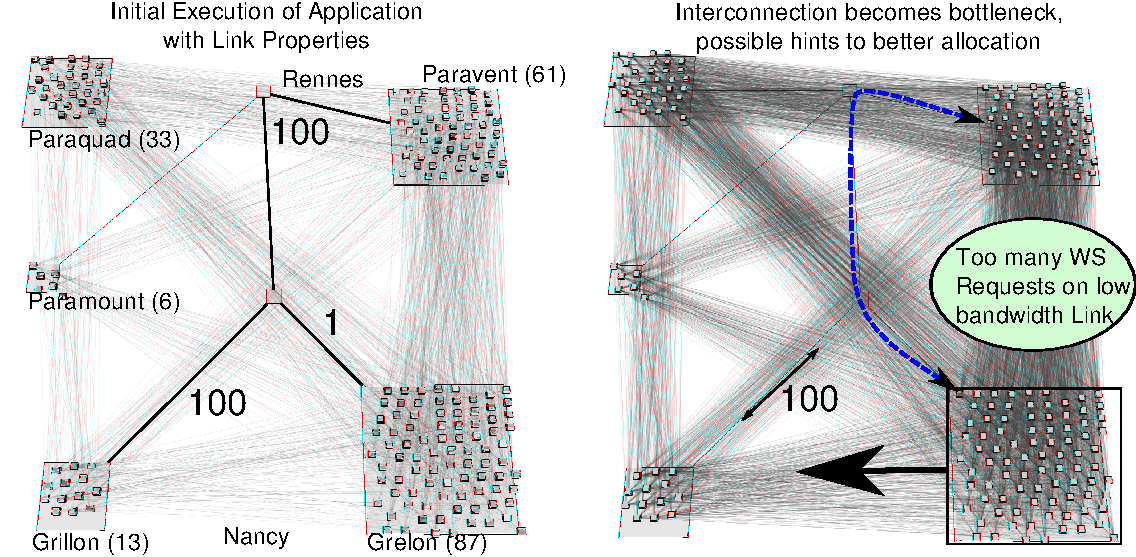
\includegraphics[width=1.15\textwidth]{img/scenario-3d-C.pdf}
   \end{minipage}
}


%\frame
%{
%   \frametitle{3D Visualization - Scenario E}
%%   \begin{itemize}
%%   \item 648 processes, two sites, five clusters
%%   \item Resulting communication pattern of KAAPI random steal requests
%%   \item Square size in the base is directly related to the number of
%%   processes in the cluster
%%   \end{itemize}
%
%   \vfill
%   \begin{center}
%   \includegraphics[width=.7\textwidth]{img/scenario-3d-D.pdf}
%   \end{center}
%}
%

\frame
{
   \frametitle{3D Visualization - KAAPI Trace}
   \begin{itemize}
   \item 2900 processes, four sites, thirteen clusters
   \end{itemize}
%   \item Illustrate different work stealing patterns that arise in different intervals of time
%   \end{itemize}
% autre façon de voir l'evolution temporelle

   \vfill
   \hspace{-1cm}
   \begin{minipage}{\textwidth}
   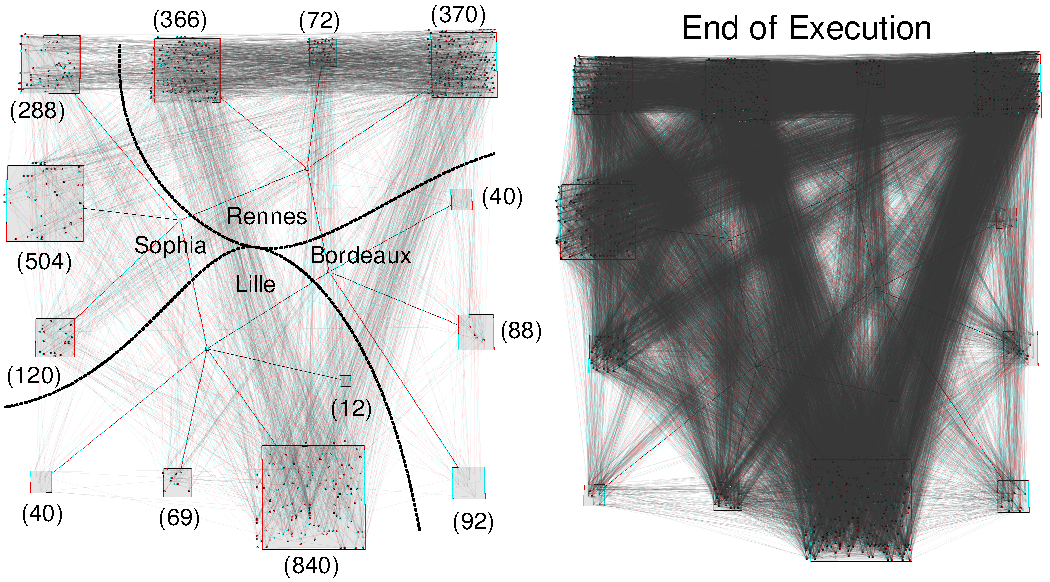
\includegraphics[width=1.15\textwidth]{img/scenario-3d-E.pdf}
   \end{minipage}
}
